\documentclass{article}
\usepackage{amsmath, amssymb} % Required for math symbols and additional symbols
\usepackage[paper=letterpaper,
           hmargin={1in,1in},
           vmargin={1in,1in},
           ]{geometry}   % Allows you to change the margin sizes
\usepackage{enumitem}  % Required to re-label lists
\usepackage{tikz}      % Required for creating graphics

\title{Prep Work 15}
\author{Xander} 
\date{Apr 15}

\begin{document}

\maketitle
\noindent\textbf{Presentation: } 


%%%%%%%%%%%%%%%%% Don't delete anything above this line!

\section*{Exercise 14 4.1}  

Consider graphs with \(n\) vertices.  Remember, graphs do not need to be \emph{connected}.%
\begin{enumerate}[label= (\alph*)]
\item{}How many edges must the graph have to guarantee at least one vertex has degree two or more?  Prove your answer.%
\item{}How many edges must the graph have to guarantee all vertices have degree two or more?  Prove your answer.%
\end{enumerate}

\vspace{0.5cm}
\noindent\textbf{Solution Draft:} 
\vspace{0.2cm}

\begin{enumerate}[label= (\alph*)]
    \item You need at least 3 edges to guarantee one vertex has degree two or more.
    
    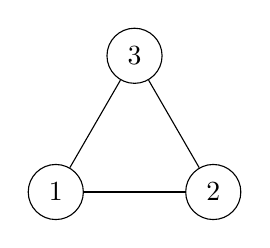
\begin{tikzpicture}
      \node[circle,draw,minimum size=0.7cm] (1) at (0,0) {1};
      \node[circle,draw,minimum size=0.7cm] (2) at (2,0) {2};
      \node[circle,draw,minimum size=0.7cm] (3) at (1,1.73) {3};
      
      \draw (1) -- (2);
      \draw (2) -- (3);
      \draw (1) -- (3);
    \end{tikzpicture}
    \item You need at leat 4 edges to guarantee all vertices have degree two or more.
    
    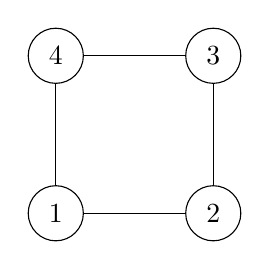
\begin{tikzpicture}
        \node[circle,draw,minimum size=0.7cm] (1) at (0,0) {1};
        \node[circle,draw,minimum size=0.7cm] (2) at (2,0) {2};
        \node[circle,draw,minimum size=0.7cm] (3) at (2,2) {3};
        \node[circle,draw,minimum size=0.7cm] (4) at (0,2) {4};
        
        \draw (1) -- (2);
        \draw (2) -- (3);
        \draw (3) -- (4);
        \draw (4) -- (1);
      \end{tikzpicture}
\end{enumerate}

%%%%%%%%%%%%%%%%%%%%%%%%%%%%%%%%%%%%
\section*{Exercise 3 4.2}  

For each degree sequence below, decide whether it must always, must never, or could possibly be a degree sequence for a tree.  Justify your answers.%
\begin{enumerate}[label= (\alph*)]
\item{}\(\displaystyle (3, 3, 2, 2, 2)\)%
\item{}\(\displaystyle (3, 2, 2, 1, 1, 1)\)%
\item{}\(\displaystyle (3, 3, 3, 1, 1, 1)\)%
\item{}\(\displaystyle (4, 4, 1, 1, 1, 1, 1, 1)\)%
\end{enumerate}

\vspace{0.5cm}
\noindent\textbf{Solution Draft:} 
\vspace{0.2cm}

A tree with $n$ vertices has $n-1$ edges.
A tree is connected and acyclic
The sum of degrees in a tree must equal $2(n-1)$.

\begin{enumerate}[label= (\alph*)]
    \item 
    Sum of degrees $3+3+2+2+2=12$

    Expected sum of a tree with 5 verticies $2*(5-1)=8$

    This sequence must never be a tree.
    \item
    Sum of degrees $3+2+2+1+1+1=10$

    Expected sum of a tree with 6 verticies $2*(6-1)=10$

    This sequence could be a tree.

    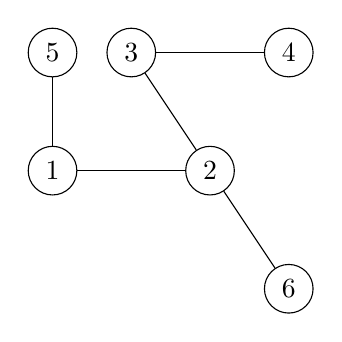
\begin{tikzpicture}
        \node[circle,draw] (1) at (0,0) {1};
        \node[circle,draw] (2) at (2,0) {2};
        \node[circle,draw] (3) at (1,1.5) {3};
        \node[circle,draw] (4) at (3,1.5) {4};
        \node[circle,draw] (5) at (0,1.5) {5};
        \node[circle,draw] (6) at (3,-1.5) {6};
      
        \draw (1) -- (2);
        \draw (2) -- (3);
        \draw (3) -- (4);
        \draw (2) -- (6);
        \draw (1) -- (5);
      \end{tikzpicture}

    \item
    Sum of degrees $3+3+3+1+1+1=12$

    Expected sum of a tree with 6 verticies $2*(6-1)=10$

    This sequence must never be a tree.

    \item
    Sum of degrees $4+4+1+1+1+1+1+1=14$

    Expected sum of a tree with 8 verticies $2*(8-1)=14$

    Even though the number of vertices lines up with the expected number for a tree. Since there are two verticies that are connected to half of the of the verticies, you cannot create this graph without a cycle.

    This sequence must never be a tree.
    \end{enumerate}

%%%%%%%%%%%%%%%%%%%%%%%%%%%%%%%%%%%%

\end{document}
